\documentclass[12 pt]{report}

\usepackage{epsfig}
\usepackage[in,empty]{myfullpage}
\usepackage{amssymb}
\usepackage{amsmath}

\baselineskip=20pt

\begin{document}

\noindent \vfill \noindent \large

\centerline{Math 324 A - Spring 2017}

\centerline{Midterm exam 1}

\centerline{Wednesday, April 19th, 2017}

\normalsize

\vfill
\medskip
Name: \rule{10cm}{1pt}

\bigskip

\vfill
\begin{center}
{\large
\begin{tabular}{||c|c|r||}
\hline Problem 1 & 10 & \hspace{10mm} \hfill \\
\hline Problem 2 & 12  & \hspace{10mm} \hfill \\
\hline Problem 3 & 16 & \hspace{10mm} \hfill \\
\hline Problem 4 & 12  & \hspace{10mm} \hfill \\
\hline Total & 50 & \hspace{10mm} \hfill \\
\hline
\end{tabular}
}
\end{center}
\vfill
\begin{itemize}
\item There are 4 questions on this exam. Make sure you have all four.
\item \textbf{You must show your work on all problems.}  The correct answer
with no supporting work may result in no credit. Put a box
around your FINAL ANSWER for each problem and cross out any work
that you don't want to be graded.
\item Give exact answers, and simplify as much as possible. 
For example, $\frac{\pi}{\sqrt{2}}$ is acceptable, but $\frac{1}{2} + \frac{3}{4}$
should be simplified to $\frac{5}{4}$.  

\item If you need more room, use the backs
of the pages and indicate to the grader that you have done so.
\item Raise your hand if you have a question.
\item Any student found engaging in academic misconduct will receive
a score of 0 on this exam.
\item You have 50 minutes to complete the exam.  Budget your time wisely! \\
\end{itemize}
\vfill
\begin{center}GOOD LUCK!\end{center}

\newpage
\begin{enumerate}

\item (10 pts) Consider the tetrahedron $E \subset \mathbb{R}^3$ bounded by the planes $x = 0, z = 0, z = 2y$ and $2x + 2y + z = 4$. Set up the triple integral 

\[
\iiint_E xz \, dV
\]

with the two given orders of integration. \textbf{You do not need to evaluate the integrals.}

\begin{enumerate} \item $dx \,dy \,dz.$
\vfill


\item $dy \, dz \, dx.$
\vfill
\end{enumerate}



\newpage

\item (12 pts) Let $R$ be the region in the plane satisfying the polar conditions $\frac{1}{2 \sin \theta} \leq r \leq \sin \theta$, and $0 \leq \theta \leq \pi/2$. 

\begin{enumerate} \item (2 pts) Draw a sketch of $R$.

\vfill

\item (4 pts) Use Cartesian coordinates -- $x$'s and $y$'s -- to set up the double integral

\[
\iint_R \sin^2 \theta \cos \theta \, dA.
\]

\textbf{You do not need to evaluate the integral.}

\vfill 

\newpage

\item (6 pts) Use polar coordinates to set up the integral from part $(b)$, and evaluate it. 

\end{enumerate}

\newpage

\item \begin{enumerate} \item (8 pts) Let $B \subset \mathbb{R}^3$ be the region inside the sphere $x^2 + y^2 + z^2 = 16$, outside the sphere $x^2 + y^2 + z^2 = 1$, and inside the cone $x^2 = 3y^2 + 3z^2$. Set up an integral to find the volume of $B$. \textbf{You do not need to evaluate it.}

\vfill

\item (8 pts) Let $S$ denote the sphere of radius $2$ centered at $(0,0,0)$, and imagine that $S$ is filled with a fluid with density function $f(x,y,z) = z^3 - z + 2$. Find the total mass of fluid inside $S$ by integrating the function $f$ over $S$. 

\vfill
\end{enumerate}


\newpage


\item (12 pts) Use the change of coordinates $x = u-2v, y = v$ to set up the integral 

$$\iint_R (x+3y) \, dA$$

in $u,v$ coordinates, where $R$ is the region in the $x-y$ plane bounded by the curves 
$$y=1, y=3, x+2y=10, x+2y=6.$$

The region $R$ is pictured below. Sketch the image region after changing coordinates, and explain how you know what the new region looks like. \textbf{You do not need to evaluate the integral.}

\flushleft 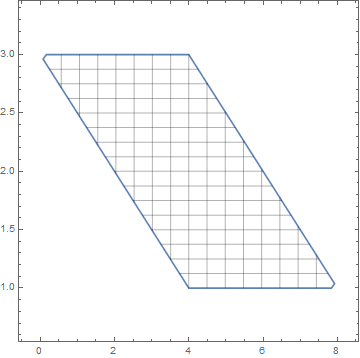
\includegraphics[width=3in]{midterm1_problem_3.png}


\end{enumerate}

\end{document}
